\chapter{Introducci\'on}
\graphicspath{{./figs/01_intro/}}
\chapterquote{La destrucción es obra de una tarde. La creación es obra de una vida.}{Kamahl, acólito druida}
\section{Motivación}\label{S:motivacion}
\cite{Mainprice2011}
\section{Difracción de Rayos X}\label{S:DRX}
Los rayos X son una herramienta de vital importancia para el estudio de los materiales cristalinos. 
En la difracción de Rayos X (DRX), un haz monocromático de de rayos X de longitud de onda $\lambda$ incide sobre una dada muestra (Fig. \ref{fig:Bragg}). 
Si el cristal es infinito y está libre de cualquier tipo de distorsiones, para una dada familia de planos ${hkl}$, habrá interferencia constructiva para los haces salientes que cumplan con la condición de Bragg[ref]:

Esto esta medio medio, hay que hablar de que los cristales estan en arreglos periodicos de atomos

\begin{equation}
  2 \ d_{hkl} \ \sin(\theta_{B}) \ = \ n \ \lambda
  \label{eq:Bragg}
\end{equation}
\noindent
siendo $d_{hkl}$ la distancia interplanar de la familia de planos $\{hkl\}$, 2$\theta_{B}$ el ángulo formado entre el haz incidente y el haz reflejado y $n$ el número de orden de difracción. 

Hay que pensar en el planteo mas riguroso, usando los vectores K, porque lo voy a necesitar para explicar williamson hall

\nomenclature{$\lambda$}{Longitud de onda}
\nomenclature{$d_{hkl}$}{Distacia interplanar para la familia de planos $hkl$}
\nomenclature{$\theta_B$}{Ángulo de Bragg}
\nomenclature{XRD}{Difracción de Rayos X}
\begin{figure}[htb!]
  \centering
  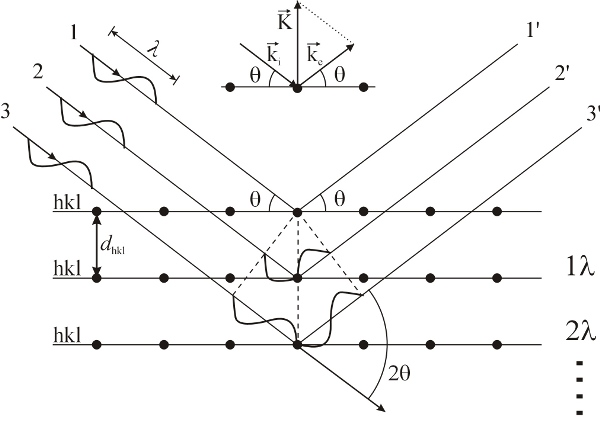
\includegraphics[width=\imsize]{BraggLaw}
  \caption{Ley de Bragg}
  \label{fig:Bragg}
\end{figure}

Una consecuencia de la ley expresada en la Ec. \ref{eq:Bragg} es que para un cierto haz incidente habrá reflexiones cuyas distribución de intensidades serán funciones deltas de Dirac[ref], con intensidad infinita para el ángulo $\theta_{B}$ e intensidad nula para los ángulos $\theta$ que no cumplan con la condición de Bragg. Como resultado, los "picos" de difracción tendrán además un ancho nulo. 
Si, como ocurre en la práctica, el número de planos que contribuyen a la reflexión es finito, la distribución angular de intensidades tendrán un ancho y altura finitos, y lo mismo ocurrirá si la red de átomos tiene distorsiones, es decir, si los átomos no se encuentran en un arreglo perfectamente periódico. 
En un experimento de DRX real aparecerán además otras contribuciones que ensancharán los picos de difracción. 
Por un lado el haz incidente no será puntual ni estará constituido por haces completamente paralelos, sino que tendrá de un tamaño finito y estará comprendido entre haces que tendrán cierta divergencia angular. 
Además, el haz no será completamente monocromático, sino que estará inegrado por rayos X con longitudes de onda en un intervalo $(\lambda \ \pm \ \Delta \lambda)$. 
Todos estos factores cotribuirán a que haya haces difractados en las vecindades de $\theta_{B}$, aumentando el ancho de los picos de difracción, y serán parte crucial de la discusión en los capítulos siguientes, ya que el ensanchamiento de los picos provee información sobre la microestructura de los materiales.

\subsection{Estudios de ancho de pico}\label{SS:DRX-LPA}
Si no se tienen en cuenta los diferentes efectos instrumentales se puede afirmar que, a partir del estudio del ensanchamiento y la forma de los perfiles de intensidad de los picos de medidos en un experimento de DRX, es posible obtener información acerca de la cantidad y tipo de defectos presentes en un material, así como información microestructural como el tamaño promedio de los dominios coherentes de difracción. 
Al conjunto de t\'ecnicas y m\'etodos del campo de la cristalografía que utilizados para obtener este tipo de información se los conoce como Estudio de Ancho de Pico, o LPA, por sus siglas en inglés (Line Profile Analysis).
Aunque el término LPA fue acuñado muchos años después, la técnica, aunque rudimentaria, es tan antigua como los primeros experimentos de DRX, y fue implementada independientemente por Hull en Estados Unidos y Debye y Scherrer en Alemania. Mientras investigaba el tamaño de partículas de oro y plata en sistemas coloidales, Scherrer incluyó la ecuación que luego llevaría su nombre[ref]:

\begin{equation}
  H \ = \ 2 \sqrt{\frac{\ln(2)}{\pi}} \ \frac{\lambda}{L \ \cos(\theta_B)}
  \label{eq:Scherrer}
\end{equation}
\noindent
Donde $H$ denota el ancho del pico a la mitad de su intensidad máxima, $L$ es la longitud característica de la cristalita y el factor numérico se usa para convertir $H$ al ancho integral del pico, suponiendo que el mismo tiene forma de gaussiana. 
Los trabajos que siguieron se dedicaron a mejorar las estimaciones de tamaño y forma de las cristalitas. 
En el año 1938 [ref] Jones señaló que el perfil de intensidades medido en un experimento de DRX, $I_{exp}$ es la convolución del perfil $I_{muestra}$ que se obtendría de la muestra y el debido a todos los efectos instrumentales, $I_{inst}$, es decir:
\begin{equation}
  I_{exp} \ = \ I_{muestra} \ \otimes \ I_{inst}
  \label{eq:conv}
\end{equation}
\noindent
De esta manera, Jones logró remover las contribuciones de las líneas $K\alpha_2$ de la radiación del cobre en las mediciones de tamaño de cristalita.


\nomenclature{$H$ o $FWHM$}{Ancho de pico a media altura. También abreviado como FWHM por sus siglas en inglés (Full Witdth at Half Maximum).}
\nomenclature{$L$}{Longitud característica de la cristalita.}

Frase de Warren?
Definicion de macro, micro, meso, nano estructura?
Diferencia entre cristalita y tamaño de grano
Definicion de defectos, dislocaciones, maclas, fallas de apilamiento, bordes de grano
Separacion, al menos en la nomenclatura de familia de planos, planos, direcciones familia de direcciones

Hay que hablar de los principios de medicion, rayos X de laboratorio y de sincrotron
Estudio de ancho de pico, Langford, Williamson Hall, Warren Averbach y CMWP

\section{Difracción de electrones retro difundidos}\label{S:EBSD}
Cómo se mide y cómo se pueden relacionar las magnitudes de EBSD con las de RX
Que permite y que no permite ver en comparacion con RX

¿Hablo de TEM?
 
\section{Textura cristalográfica}\label{S:Text}
Definicion de textura, relacion con los procesos de deformacion y la microestructura.
ODF: definicion y obtencion a partir de RX y EBSD. Diferencias de los dos métodos.

\subsection{FDO y FDO generalizada}\label{SS:ODF}
Relacion entre la ODF y la ODF generalizada. Relacion de FWHM y energía de deformacion.

\section{Revisión bibliográfica y estado del arte}\label{S:RB}

\section{Organización de la tesis}\label{S:Org}
